
%% capstone.tex
%% V1.4
%% 2012/12/27
%% by Michael Shell
%% See:
%% http://www.michaelshell.org/
%% for current contact information.
%%
%% This is a skeleton file demonstrating the use of IEEEtran.cls
%% (requires IEEEtran.cls version 1.8 or later) with an IEEE conference paper.
%%
%% Support sites:
%% http://www.michaelshell.org/tex/ieeetran/
%% http://www.ctan.org/tex-archive/macros/latex/contrib/IEEEtran/
%% and
%% http://www.ieee.org/

%%*************************************************************************
%% Legal Notice:
%% This code is offered as-is without any warranty either expressed or
%% implied; without even the implied warranty of MERCHANTABILITY or
%% FITNESS FOR A PARTICULAR PURPOSE! 
%% User assumes all risk.
%% In no event shall IEEE or any contributor to this code be liable for
%% any damages or losses, including, but not limited to, incidental,
%% consequential, or any other damages, resulting from the use or misuse
%% of any information contained here.
%%
%% All comments are the opinions of their respective authors and are not
%% necessarily endorsed by the IEEE.
%%
%% This work is distributed under the LaTeX Project Public License (LPPL)
%% ( http://www.latex-project.org/ ) version 1.3, and may be freely used,
%% distributed and modified. A copy of the LPPL, version 1.3, is included
%% in the base LaTeX documentation of all distributions of LaTeX released
%% 2003/12/01 or later.
%% Retain all contribution notices and credits.
%% ** Modified files should be clearly indicated as such, including  **
%% ** renaming them and changing author support contact information. **
%%
%% File list of work: IEEEtran.cls, IEEEtran_HOWTO.pdf, bare_adv.tex,
%%                    bare_conf.tex, bare_jrnl.tex, bare_jrnl_compsoc.tex,
%%                    bare_jrnl_transmag.tex
%%*************************************************************************

% *** Authors should verify (and, if needed, correct) their LaTeX system  ***
% *** with the testflow diagnostic prior to trusting their LaTeX platform ***
% *** with production work. IEEE's font choices can trigger bugs that do  ***
% *** not appear when using other class files.                            ***
% The testflow support page is at:
% http://www.michaelshell.org/tex/testflow/



% Note that the a4paper option is mainly intended so that authors in
% countries using A4 can easily print to A4 and see how their papers will
% look in print - the typesetting of the document will not typically be
% affected with changes in paper size (but the bottom and side margins will).
% Use the testflow package mentioned above to verify correct handling of
% both paper sizes by the user's LaTeX system.
%
% Also note that the "draftcls" or "draftclsnofoot", not "draft", option
% should be used if it is desired that the figures are to be displayed in
% draft mode.
%
\documentclass[conference]{IEEEtran}

% Add the compsoc option for Computer Society conferences.
%
% If IEEEtran.cls has not been installed into the LaTeX system files,
% manually specify the path to it like:
% \documentclass[conference]{../sty/IEEEtran}





% Some very useful LaTeX packages include:
% (uncomment the ones you want to load)


% *** MISC UTILITY PACKAGES ***
%
%\usepackage{ifpdf}
% Heiko Oberdiek's ifpdf.sty is very useful if you need conditional
% compilation based on whether the output is pdf or dvi.
% usage:
% \ifpdf
%   % pdf code
% \else
%   % dvi code
% \fi
% The latest version of ifpdf.sty can be obtained from:
% http://www.ctan.org/tex-archive/macros/latex/contrib/oberdiek/
% Also, note that IEEEtran.cls V1.7 and later provides a builtin
% \ifCLASSINFOpdf conditional that works the same way.
% When switching from latex to pdflatex and vice-versa, the compiler may
% have to be run twice to clear warning/error messages.






% *** CITATION PACKAGES ***
%
%\usepackage{cite}
% cite.sty was written by Donald Arseneau
% V1.6 and later of IEEEtran pre-defines the format of the cite.sty package
% \cite{} output to follow that of IEEE. Loading the cite package will
% result in citation numbers being automatically sorted and properly
% "compressed/ranged". e.g., [1], [9], [2], [7], [5], [6] without using
% cite.sty will become [1], [2], [5]--[7], [9] using cite.sty. cite.sty's
% \cite will automatically add leading space, if needed. Use cite.sty's
% noadjust option (cite.sty V3.8 and later) if you want to turn this off
% such as if a citation ever needs to be enclosed in parenthesis.
% cite.sty is already installed on most LaTeX systems. Be sure and use
% version 4.0 (2003-05-27) and later if using hyperref.sty. cite.sty does
% not currently provide for hyperlinked citations.
% The latest version can be obtained at:
% http://www.ctan.org/tex-archive/macros/latex/contrib/cite/
% The documentation is contained in the cite.sty file itself.






% *** GRAPHICS RELATED PACKAGES ***
%
\ifCLASSINFOpdf
  \usepackage[pdftex]{graphicx}
  % declare the path(s) where your graphic files are
  \graphicspath{{../pdf/}{../figs/}}
  % and their extensions so you won't have to specify these with
  % every instance of \includegraphics
  \DeclareGraphicsExtensions{.pdf,.jpeg,.png}
\else
  % or other class option (dvipsone, dvipdf, if not using dvips). graphicx
  % will default to the driver specified in the system graphics.cfg if no
  % driver is specified.
  % \usepackage[dvips]{graphicx}
  % declare the path(s) where your graphic files are
  % \graphicspath{{../eps/}}
  % and their extensions so you won't have to specify these with
  % every instance of \includegraphics
  % \DeclareGraphicsExtensions{.eps}
\fi
% graphicx was written by David Carlisle and Sebastian Rahtz. It is
% required if you want graphics, photos, etc. graphicx.sty is already
% installed on most LaTeX systems. The latest version and documentation
% can be obtained at: 
% http://www.ctan.org/tex-archive/macros/latex/required/graphics/
% Another good source of documentation is "Using Imported Graphics in
% LaTeX2e" by Keith Reckdahl which can be found at:
% http://www.ctan.org/tex-archive/info/epslatex/
%
% latex, and pdflatex in dvi mode, support graphics in encapsulated
% postscript (.eps) format. pdflatex in pdf mode supports graphics
% in .pdf, .jpeg, .png and .mps (metapost) formats. Users should ensure
% that all non-photo figures use a vector format (.eps, .pdf, .mps) and
% not a bitmapped formats (.jpeg, .png). IEEE frowns on bitmapped formats
% which can result in "jaggedy"/blurry rendering of lines and letters as
% well as large increases in file sizes.
%
% You can find documentation about the pdfTeX application at:
% http://www.tug.org/applications/pdftex





% *** MATH PACKAGES ***
%
%\usepackage[cmex10]{amsmath}
% A popular package from the American Mathematical Society that provides
% many useful and powerful commands for dealing with mathematics. If using
% it, be sure to load this package with the cmex10 option to ensure that
% only type 1 fonts will utilized at all point sizes. Without this option,
% it is possible that some math symbols, particularly those within
% footnotes, will be rendered in bitmap form which will result in a
% document that can not be IEEE Xplore compliant!
%
% Also, note that the amsmath package sets \interdisplaylinepenalty to 10000
% thus preventing page breaks from occurring within multiline equations. Use:
%\interdisplaylinepenalty=2500
% after loading amsmath to restore such page breaks as IEEEtran.cls normally
% does. amsmath.sty is already installed on most LaTeX systems. The latest
% version and documentation can be obtained at:
% http://www.ctan.org/tex-archive/macros/latex/required/amslatex/math/





% *** SPECIALIZED LIST PACKAGES ***
%
%\usepackage{algorithmic}
% algorithmic.sty was written by Peter Williams and Rogerio Brito.
% This package provides an algorithmic environment fo describing algorithms.
% You can use the algorithmic environment in-text or within a figure
% environment to provide for a floating algorithm. Do NOT use the algorithm
% floating environment provided by algorithm.sty (by the same authors) or
% algorithm2e.sty (by Christophe Fiorio) as IEEE does not use dedicated
% algorithm float types and packages that provide these will not provide
% correct IEEE style captions. The latest version and documentation of
% algorithmic.sty can be obtained at:
% http://www.ctan.org/tex-archive/macros/latex/contrib/algorithms/
% There is also a support site at:
% http://algorithms.berlios.de/index.html
% Also of interest may be the (relatively newer and more customizable)
% algorithmicx.sty package by Szasz Janos:
% http://www.ctan.org/tex-archive/macros/latex/contrib/algorithmicx/




% *** ALIGNMENT PACKAGES ***
%
%\usepackage{array}
% Frank Mittelbach's and David Carlisle's array.sty patches and improves
% the standard LaTeX2e array and tabular environments to provide better
% appearance and additional user controls. As the default LaTeX2e table
% generation code is lacking to the point of almost being broken with
% respect to the quality of the end results, all users are strongly
% advised to use an enhanced (at the very least that provided by array.sty)
% set of table tools. array.sty is already installed on most systems. The
% latest version and documentation can be obtained at:
% http://www.ctan.org/tex-archive/macros/latex/required/tools/


% IEEEtran contains the IEEEeqnarray family of commands that can be used to
% generate multiline equations as well as matrices, tables, etc., of high
% quality.




% *** SUBFIGURE PACKAGES ***
%\ifCLASSOPTIONcompsoc
%  \usepackage[caption=false,font=normalsize,labelfont=sf,textfont=sf]{subfig}
%\else
%  \usepackage[caption=false,font=footnotesize]{subfig}
%\fi
% subfig.sty, written by Steven Douglas Cochran, is the modern replacement
% for subfigure.sty, the latter of which is no longer maintained and is
% incompatible with some LaTeX packages including fixltx2e. However,
% subfig.sty requires and automatically loads Axel Sommerfeldt's caption.sty
% which will override IEEEtran.cls' handling of captions and this will result
% in non-IEEE style figure/table captions. To prevent this problem, be sure
% and invoke subfig.sty's "caption=false" package option (available since
% subfig.sty version 1.3, 2005/06/28) as this is will preserve IEEEtran.cls
% handling of captions.
% Note that the Computer Society format requires a larger sans serif font
% than the serif footnote size font used in traditional IEEE formatting
% and thus the need to invoke different subfig.sty package options depending
% on whether compsoc mode has been enabled.
%
% The latest version and documentation of subfig.sty can be obtained at:
% http://www.ctan.org/tex-archive/macros/latex/contrib/subfig/




% *** FLOAT PACKAGES ***
%
%\usepackage{fixltx2e}
% fixltx2e, the successor to the earlier fix2col.sty, was written by
% Frank Mittelbach and David Carlisle. This package corrects a few problems
% in the LaTeX2e kernel, the most notable of which is that in current
% LaTeX2e releases, the ordering of single and double column floats is not
% guaranteed to be preserved. Thus, an unpatched LaTeX2e can allow a
% single column figure to be placed prior to an earlier double column
% figure. The latest version and documentation can be found at:
% http://www.ctan.org/tex-archive/macros/latex/base/


%\usepackage{stfloats}
% stfloats.sty was written by Sigitas Tolusis. This package gives LaTeX2e
% the ability to do double column floats at the bottom of the page as well
% as the top. (e.g., "\begin{figure*}[!b]" is not normally possible in
% LaTeX2e). It also provides a command:
%\fnbelowfloat
% to enable the placement of footnotes below bottom floats (the standard
% LaTeX2e kernel puts them above bottom floats). This is an invasive package
% which rewrites many portions of the LaTeX2e float routines. It may not work
% with other packages that modify the LaTeX2e float routines. The latest
% version and documentation can be obtained at:
% http://www.ctan.org/tex-archive/macros/latex/contrib/sttools/
% Do not use the stfloats baselinefloat ability as IEEE does not allow
% \baselineskip to stretch. Authors submitting work to the IEEE should note
% that IEEE rarely uses double column equations and that authors should try
% to avoid such use. Do not be tempted to use the cuted.sty or midfloat.sty
% packages (also by Sigitas Tolusis) as IEEE does not format its papers in
% such ways.
% Do not attempt to use stfloats with fixltx2e as they are incompatible.
% Instead, use Morten Hogholm'a dblfloatfix which combines the features
% of both fixltx2e and stfloats:
%
% \usepackage{dblfloatfix}
% The latest version can be found at:
% http://www.ctan.org/tex-archive/macros/latex/contrib/dblfloatfix/




% *** PDF, URL AND HYPERLINK PACKAGES ***
%
%\usepackage{url}
% url.sty was written by Donald Arseneau. It provides better support for
% handling and breaking URLs. url.sty is already installed on most LaTeX
% systems. The latest version and documentation can be obtained at:
% http://www.ctan.org/tex-archive/macros/latex/contrib/url/
% Basically, \url{my_url_here}.




% *** Do not adjust lengths that control margins, column widths, etc. ***
% *** Do not use packages that alter fonts (such as pslatex).         ***
% There should be no need to do such things with IEEEtran.cls V1.6 and later.
% (Unless specifically asked to do so by the journal or conference you plan
% to submit to, of course. )


% correct bad hyphenation here
\hyphenation{op-tical net-works semi-conduc-tor}
\usepackage{float}

\begin{document}
%
% paper title
% can use linebreaks \\ within to get better formatting as desired
% Do not put math or special symbols in the title.
\title{Attack Surface Measurement on Android Applications}


% author names and affiliations
% use a multiple column layout for up to three different
% affiliations
\author{\IEEEauthorblockN{Kevin Campusano}
\IEEEauthorblockA{B. Thomas Golisano College of Computing and Information Sciences\\
Rochester Institute of Technology\\
Rochester, New York 14623\\
Email: kac2375@rit.edu\\
Advisor: Dr. Andy Meneely}}

% conference papers do not typically use \thanks and this command
% is locked out in conference mode. If really needed, such as for
% the acknowledgment of grants, issue a \IEEEoverridecommandlockouts
% after \documentclass

% for over three affiliations, or if they all won't fit within the width
% of the page, use this alternative format:
% 
%\author{\IEEEauthorblockN{Michael Shell\IEEEauthorrefmark{1},
%Homer Simpson\IEEEauthorrefmark{2},
%James Kirk\IEEEauthorrefmark{3}, 
%Montgomery Scott\IEEEauthorrefmark{3} and
%Eldon Tyrell\IEEEauthorrefmark{4}}
%\IEEEauthorblockA{\IEEEauthorrefmark{1}School of Electrical and Computer Engineering\\
%Georgia Institute of Technology,
%Atlanta, Georgia 30332--0250\\ Email: see http://www.michaelshell.org/contact.html}
%\IEEEauthorblockA{\IEEEauthorrefmark{2}Twentieth Century Fox, Springfield, USA\\
%Email: homer@thesimpsons.com}
%\IEEEauthorblockA{\IEEEauthorrefmark{3}Starfleet Academy, San Francisco, California 96678-2391\\
%Telephone: (800) 555--1212, Fax: (888) 555--1212}
%\IEEEauthorblockA{\IEEEauthorrefmark{4}Tyrell Inc., 123 Replicant Street, Los Angeles, California 90210--4321}}




% use for special paper notices
%\IEEEspecialpapernotice{(Invited Paper)}




% make the title area
\maketitle

% As a general rule, do not put math, special symbols or citations
% in the abstract
% \begin{abstract}
% The abstract goes here.
% \end{abstract}

% no keywords




% For peer review papers, you can put extra information on the cover
% page as needed:
% \ifCLASSOPTIONpeerreview
% \begin{center} \bfseries EDICS Category: 3-BBND \end{center}
% \fi
%
% For peerreview papers, this IEEEtran command inserts a page break and
% creates the second title. It will be ignored for other modes.
\IEEEpeerreviewmaketitle



\section{Introduction}
% no \IEEEPARstart
Mobile devices have seen an explosive increment in use during the past few years. With the advent of tablets, phones and other smart devices, computing has taken a new, more accessible and portable form and has become integral to our everyday lives now more than ever. With processing power comparable to conventional desktop machines, these devices are capable of meeting our most common computing needs. To achieve this, smart devices access and manipulate sensitive information such as location, calendars and emails. Indeed, smart devices provide a lot of convenience. However, due to the amount of sensitive information they manage, they also represent a security risk.

In this day and age only a handful of different mobile platforms hold the majority of the market share. Among those, Android has seen an outstanding growth in its install base and now holds a privileged position of more than half of smartphone users in the US \cite{_android_news}. Due in part to its popularity, the Android platform has been the target of multiple attacks \cite{vidas_all_2011}. Even though Android's application development framework and the operating system itself provide (although not perfect \cite{shabtai_google_2010}) many defense mechanisms \cite{burns2009mobile} \cite{enck2011study}, the responsibility to protect sensitive information ultimately falls to application developers as their applications are what interact directly with the users and their information.

With security being such an important concern, the need for it to be managed is imperative. For software security to be managed and subsequently improved, measuring it, as is the case with most quality attributes, is essential. To address this problem we propose the use of a measurement of applications' attack surface based on their call graph information \cite{Manadhata2011AnAttackSurfaceMetric}.

The attack surface is defined as all the different ways in which a malicious user can take advantage of a system and compromise its data. It can be thought as the “attackability” of a system. We can say then, that the smaller a system's attack surface is, the more secure it is \cite{Manadhata2011AnAttackSurfaceMetric}. It makes sense then that a metric for the attack surface would be relative. As such, we propose measuring the attack surface of different versions of an application and comparing the various measurements to discover its evolution and whether it has become “more” or “less” secure.

To guide our research efforts, we propose the following research questions:

\begin{itemize}
  \item Can the attack surface of an Android application be measured?
  \item How does the attack surface evolve in Android applications?
\end{itemize}

Past research in the area of Android application security has focused on enhancements to the application development framework's security aspects \cite{ongtang_semantically_2012}, application privilege \cite{bugiel2012towards} and inter-application communication \cite{chin_analyzing_2011}. There has been previous work on attack surface of android \cite{bartel_automatically_2012} that used call graph information of applications to identify permission gaps. Our approach proposes the use of call graph information to measure and characterize the attack surface and use this to observe the difference in security between various versions of studied applications.

\section{Android Application Development Platform Overview}

The Android platform provides developers with a rich application development framework that contains a varied collection of libraries for most common functionalities and for interaction with the device's physical components. This development framework provides a core set of building blocks that most Android applications are constructed with:

\subsection{Activities}

The most common of the framework's main building blocks. All applications that involve some sort of interaction with the user are composed of at least one Activity. Activities are what provide user interfaces for the applications. In a traditional sense, each activity would correspond to a “screen”, so to speak. They contain both graphical user interface definitions and code.

\subsection{Services}

Services embody operations that run in the background without any interaction with the user. Downloading a file or continuously keeping email synchronized are some examples of functionalities that are typically implemented as services.

\subsection{Broadcast Receivers}

These are components that are responsible of receiving messages (i.e. Intents) from other applications or services that are intended to be handled for multiple applications. More often than not, a Broadcast Receiver's sole purpose is to relay the received messages to an Activity or Service that supports the particular operation specified in the Intent.

\subsection{Content Providers}

These are shared storage resources that can be accessed by multiple applications using their assigned URIs. These are used for both data persistence and information sharing between apps.

\subsection{Intents}

Android's inter process communication mechanisms are built around Intents. These are objects that encapsulate a message which typically contains a recipient, an operation and some data to work with. Intents can be sent both from the operating system and applications and can be handled by Activities, Services and Broadcast Receivers.

Depending on how the recipient for the operation described in the intent is specified, these can be of two types: Explicit and Implicit. Explicit Intents specify their recipient application while the Implicit ones describe their recipient as any application that meets certain criteria (i.e. that support the operation that the Intent represents). Implicit Intents rely on the Android platform to find a suitable application to handle it. The operating system also allows the user to select which application to handle such operations if multiple applications that support that functionality are installed in the device.

\section{Android Security Model Overview}

Android is in essence a linux based operating system build from the ground up with a focus on mobile devices and security as one of its main design goals. As such, there are security mechanisms put in place at the operating system level that affect how the users interact with their devices.

\subsection{The Market}

There are many different virtual markets from where users can obtain Android applications. The biggest one of these is the Google Play store. One of the core objectives of the Android platform is to keep it accessible both to developers and users. The process of getting applications in the store is simple and the cost is minimal. While this strategy is sound for ensuring the growth and relevance of the platform, it is not as sound for security purposes. Ill intentioned developers won't find much resistance in getting malicious applications into the Android market which will subsequently reach consumer devices and potentially compromise them and their users' data.

\subsection{Permissions}

Android's security model is permission based. This means that the concept of permissions plays an integral role in the security of the platform. These permissions are what control the applications' access to the user's personal data store in the device as well as access to any physical component on the device. Android permissions range from access to the user's contacts information to the ability to use of the camera installed in the device.

Prior to installing an application, the underlying operating system prompts the user with the permissions that the application about to be installed requires to function. The user has the option to accept or decline installing the application after (hopefully) carefully reviewing the permissions requested. These permissions are specified by the developers as part of the application's source files.

\subsection{Runtime}

At runtime, all the applications that are installed in the device are executed in isolation. The kernel provides a sandboxing mechanism that allows the applications to run separate to each other and to the rest of the system functions. In their sandbox, each application has its own set of resources that are not shared with any other running process. Each application runs in a different instance of the interpreter. 

This design prevents any application from accessing private data from the system and from other applications.

\subsection{Inter-application Communication}

Even though, by design, applications run in isolation in the Android platform, there are mechanisms for interprocess communication in place. In Android, interprocess communication is achieved by one of the basic building blocks of the Android application development framework: Intents. Intents are objects that can be instantiated by any application and the operating system itself and encapsulate a message that can be sent to other running processes. This message generally contains information for the receiver about what operation to perform, what data to work with or both.

When Intents are sent, they can be directed to a specific application or to any application that supports handling the particular action specified in the Intent. For example, an application that requires the camera may not directly use it but invoke the default camera application installed in the device. For this, the requesting application will create an Intent and configure it to be handled by the camera application. Likewise, the operating system could use Intents to notify a power saving application when the battery life has reached a certain threshold of consumption.

\section{Related Work}

There has been extensive work in the area of security in the Android platform. 

\subsection{Android Security}

Shabtai et al. \cite{shabtai_google_2010} performed a comprehensive security assessment of the Android platform. They evaluated all security concepts and mechanisms used in the platform. Both those that are inherited from the Linux kernel and new to the Android operating system itself. They identified potential weaknesses on the security mechanisms of the platform and offered several techniques that could be used to address these weaknesses. 

Gommerstadt et al. \cite{gommerstadt2012android} developed a model of the information flow in Android applications with a focus on the flow of private and sensitive data. They use previous studies on Android security as a base for their model and present two applications as case studies as a way for using their model to study the flow of information.

\subsection{Taxonomy of Android Attacks}

Vidas et al. \cite{vidas_all_2011} from the Carnegie Mellon University developed a taxonomy of all the known attacks that targeted the Android platform. The classification they proposed grouped the attack classes into two categories depending on the access that the attacker would need on the device: Attacks with physical access and attacks with no physical access.

\subsubsection{Attacks without physical access}

For these types of attacks, the attacker need not have physical access to the targeted device. Generally, these attacks consist on the attacker finding the way to execute malicious code on the device. In essence, this means that the attacker convinces the user to trust and run their code one way or the other. Once the malicious code is running on the targeted device, any vulnerability can be exploited to obtain privileged access and compromise the user's sensitive data or cause other manners of harm.

\textbf{Unprivileged Attacks}: Although the way that most attacks can maximize the damage they cause in a device is by obtaining elevated privileges, there is still fair amount of harm that can be done without breaking free from the Android security model. Still within their sandbox, with standard application permissions, malware can be dangerous. 

Some of the ways that seemingly benign applications can reach a user's device is by installing them directly from the Internet bypassing and ignoring any operating system warning as well as installing applications that request a large number of permissions at install time with dubious purposes. The Google Play Store as well as many other Android markets provide a web based interface that users can use to remotely install applications to their devices. If an attacker were to somehow hijack the user's session or authentication credentials, then they would have the ability to install any malicious application to the user's device and potentially compromise it. In addition to these methods, application repacking is a threat present in Android markets. Application repacking consists on the attacker downloading and decompiling existing popular applications, injecting malicious code into them and reuploading them to the market. Since these repacked applications are identical to their legitimate counterparts, users are tricked into installing them without a second thought and subsequently running malicious code on their device.

\textbf{Privileged Attacks}: Attacks consisting on obtaining elevated privileges and remotely executing code are based on many of the same techniques discussed earlier. The attacker somehow finds a way to get malicious code to execute on the targeted device, the difference is that this code's purpose is to perform a privilege escalation attack. Code that executes with elevated privilege in the device is outside the restrictions of all of the platform's security mechanisms and as such has a great potential of causing harm.

These kinds of remote exploitation attacks can also be achieved without the installation of malicious software in the target device. Vulnerabilities in common software that mobile devices use like web browsers or even the underlying Linux kernel can be exploited to run harmful code with high privilege.

Bugiel et al \cite{bugiel2012towards} explore the problem of developing a framework to protect the Android platform against two specific types of privilege escalation attacks: confused deputy and collusion attacks. They contribute with ways to improve the security of Android against these types of attacks.

\subsubsection{Attacks with physical access}

Of course, physical security is still a valid concern. This category describes the attacks that can be done when the attacker obtains physical access to the device.

\textbf{ADB enabled}: The Android Developer Bridge is a program that aids in the development and debugging of Android applications from a computer connected to a device. If an attacker gains physical access to a device where the Android Developer Bridge is enabled they can hook it up to a computer that has the Android developer tools installed and interact with the device. This can be done even if the device is obstructed with mechanisms such as lock screens. Via the ADB, the attacker is able to run untrusted code in the device and, as a consequence, compromise user information. Privilege escalation attacks can also be performed this same way by running the exploits from the ADB.

\textbf{ADB disabled}: If an attacker gains access to a device that is obstructed and in which the ADB is disabled, there are still options available to take advantage of it. The way to attack such a device is by booting the device in recovery mode using a forged recovery image. When booting from this image, the attacker has total control over the device and can run malicious code or gain elevated privileges.

\textbf{On unobstructed devices}: This is the best case scenario for the attacker. If the attacker gains physical access to an unattended device that is not obstructed in any way (e.g. no screen lock) then the effort needed to run malicious code in it is minimal. In this situation any of the previously discussed attack methods are available.

Based on their proposed taxonomy and the attacker's capabilities, Vidas et al. also designed a flowchart of how an attacker would approach a breach into an Android system. It can be seen in Figure \ref{fig:attackflow}.

\begin{figure}
  \centering
  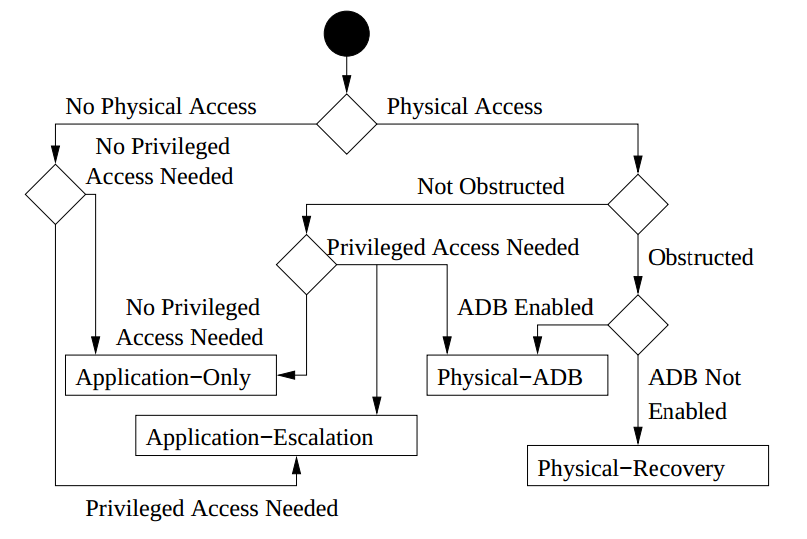
\includegraphics[scale=0.30]{figs/attackflow.png}
  \caption{Android attack flowchart developed by Vidas et al.}
  \label{fig:attackflow}
\end{figure}

\subsection{The Attack Surface}

As Manadhata and Wing \cite{Manadhata2011AnAttackSurfaceMetric} put it: "A system's attack surface is the subset of its resources that an attacker can use to attack the system." In their work Manadhata et al. \cite{Manadhata2011AnAttackSurfaceMetric} come up with a definition for a multi-dimensional metric for attack surfaces based on many factors. One particularly important is the count of Entry and Exit Points of the system under analysis. They develop a methodology for obtaining systems' Entry and Exit Points based on their call graph. Both static (compile-time) and dynamic (runtime) data is needed for a comprehensive call graph.

In subsequent work, Manadhata et al. \cite{manadhata_measuring_2006} \cite{manadhata2009report} use their developed methodology to measure and study the attack surface of industrial and open source software. In  \cite{manadhata_measuring_2006} they present a case study on two applications in the same domain. The authors apply the concepts explored in their previous work and put them to practice with two case studies. They use their multi-dimensional attack surface metric to compare the security attribute of two Unix FTP Daemons: ProFTPD and WuFTPD. This paper provides a real-world scenario in which an attack surface metric could be used to support software acquisition decisions by comparing the attack surface of two or more software alternatives.

In \cite{manadhata2009report} they present another case study, this time with an enterprise software written in Java: SAP. They implement their metric calculation methodology as an eclipse IDE plugin. In this case study, they present their metric as a complementary approach to general code quality assessments for software security.

\subsection{The Attack Surface in Android}

Previous work on attack surface of Android applications has focused on inter-application communication \cite{chin_analyzing_2011} and permission gaps \cite{bartel_automatically_2012}. Bartel et al. \cite{bartel_automatically_2012} focus on the “permission-gap” and uses that to define the attack surface in Android applications. They define this as the mismatch between the permissions that an application requests at installation-time and the ones that it actually uses. Their premise is that the bigger the difference between permissions quantity the larger the attack surface because there are more permissions requested but not needed. They develop a static analysis based method to extracting the call graph information of Android applications calculate their permission gap.

Chin et al. \cite{chin_analyzing_2011} explore another aspect of Android applications' security related to the attack surface: inter-application communication. They explain the risks that come with inter-application communication and present a tool they developed to analyze applications and detect vulnerabilities.

Our approach proposes the use of call graph information to measure and characterize the attack surface and use this to observe the difference in security between various versions of applications.

\section{Methodology}

\begin{figure*}
  \centering
  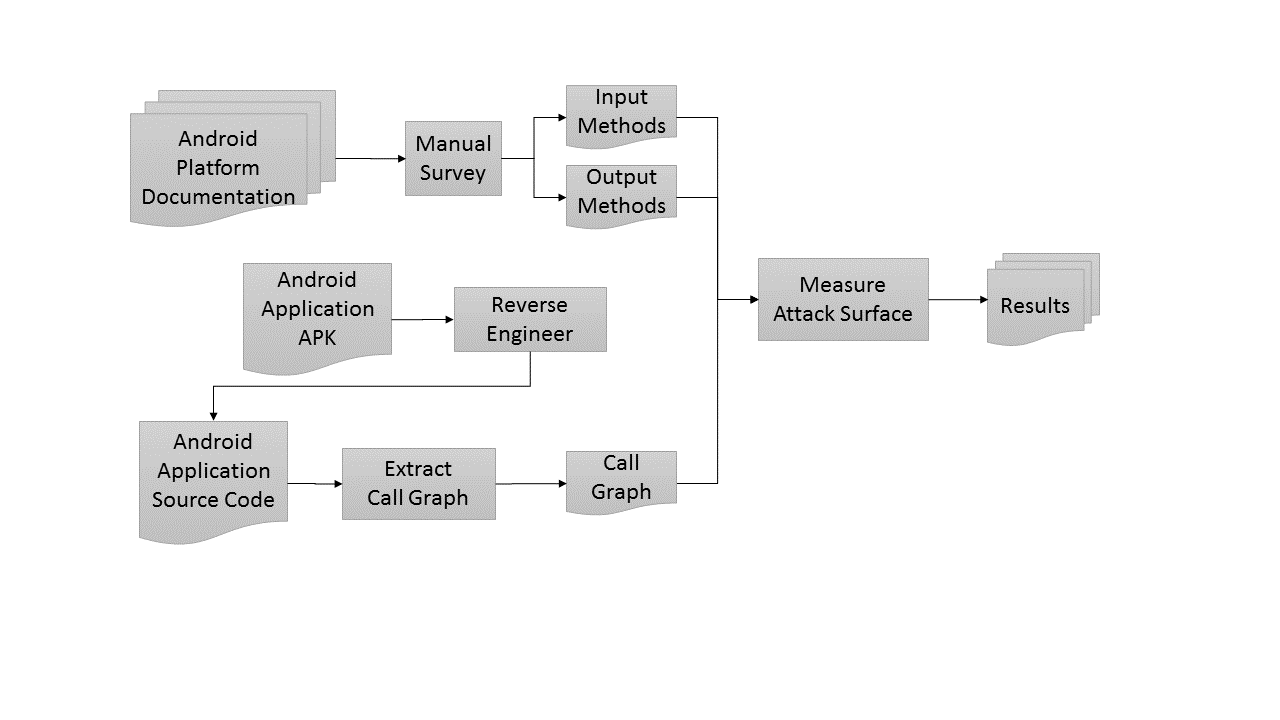
\includegraphics[scale=0.45]{figs/methodology.png}
  \caption{Overview of the attack Surface measurement methodology}
  \label{fig:methodology}
\end{figure*}

In our study, we plan to develop a method for measuring the attack surface of Android applications based on Entry Points and Exit Points obtained from their call graph information. By definition, Entry Points are the functions, methods or procedures through which data flows into the system. Similarly, Exit points are those through which data flows out of the system. Simply put, Entry Points are methods that contain calls to APIs for data input (i.e. Input Methods) and Exit Points are methods that contain calls to APIs for data output (i.e. Output Methods). The basic process for measuring the attack surface in terms of Entry Points and Exit Points involves obtaining the applications call graph from the source code and identifying all the Entry and Exit points in the call graph.

The initial efforts in this project will be geared towards building knowledge about the Android platform that will allow us to obtain the call graph and identify the Entry and Exit Points. The first step of our study will be to survey the Android application development framework and identify all the Input and Output Methods present in the libraries. These Input and Output Methods will serve as a basis for identifying the Entry and Exit Points once the call graph is obtained. As a result of this step, we expect to have a list of all the Input and Output Methods that can be programmatically used to identify Entry and Exit Points given a particular call graph.

During this step we will also look for tools that will allow us to obtain the call graph of Android applications. Given prior experience, we expect these tools to rely on either source code static analysis or runtime monitoring of executing applications. A combination of the two approaches may be necessary to obtain a comprehensive call graph. In our approach, the soundness of the call graph is essential to the measurement of the attack surface.

After this, the next step would be to use this knowledge to implement an automated tool that will allow us to, given an application's source code, invoke the call graph generation utilities discussed earlier and parse whatever output format we obtain from them and turn it into an in-memory data structure that can be operated on to obtain a diverse set of metrics based on graph analysis.

When the tool has been successfully developed and tested, we will proceed to obtain the source code of a variety of Android applications and measure their attack surface. Figure \ref{fig:methodology} shows an overview of the proposed methodology for attack surface measurement. We plan to divide this stage of the study into two phases: with the majority of the applications we will perform a single measurement and on a select few we will delve in more deeply and perform an evolution analysis. some of the applications we select as case studies will be analyzed with more depth by observing the change attack surface across releases. For this, we will obtain the source code of said applications as they were at different points in time and make our measurements on these code bases.

To maximize our sample, we will obtain the case study applications' source code by downloading the installation packages (i.e. APKs) from the Google Play Store (or any other Android store) and decompiling them. This way we won't be limited by the availability of open source applications. For our evolutionary analysis, however, we will still need access to the source code repositories of the applications we select to perform this study on. Hence, we will be limited to open source applications for this more detailed study.

\section{Tools}

\textbf{Python}: The Python \cite{python_lang} programming language will be used for developing the scripts and tools needed for measuring the attack surface. In previous work, we have developed a tool that, given an in-memory representation of a call graph, calculates various metrics. We plan to extend this tool with support for Android applications. For this we will need to develop an Android call graph parser component that will take a text representation of the call graph on an application and convert it to an in-memory data structure that can be operated on. Other enhancements will need to be done in order to support the new Entry and Exit Points definitions that will be derived from studying the Android application development framework.

\textbf{Networkx}: Networkx \cite{networkx_lib} is a Python library that offers graph analysis functionalities. Once the call graph is translated into a data structure that Networkx can work with, it will be used to calculate various types of metrics.

\textbf{Git}: The applications that we select for performing the evolutionary analysis will most likely have their source code version controlled in Git \cite{git_scm}. We will use the many features provided by the Git command line interface to mine the repositories and obtain multiple versions of the applications we select as case studies for the evolutionary analysis.

\textbf{android-apktool}: This tool \cite{android_apktool} will allow us to reverse engineer the Android application packages (APKs) containing the applications that we select as case studies and obtain their source code for analysis.

\textbf{java-callgraph}: We will use this tool \cite{java_callgraph} to obtain the call graph information of the android applications we select as case studies.

\textbf{Spark}: An alternative call graph generation tool for java that is part of the Soot analysis framework \cite{soot_framework} \cite{Lam_thesoot}.

\section{Work Schedule}

\begin{table*}[!t]
\renewcommand{\arraystretch}{1.3}
\caption{Project Work Schedule}
\label{tab:schedule}
\centering
\begin{tabular}{|l|c|c|}
\hline
Activity & Begin & End \\
\hline
Android Platform study & 2/2/2015 & 2/20/2015 \\ 
\hline 
Entry/Exit Point definition development & 2/9/2015 & 2/20/2015 \\
\hline 
APK reverse engineering tool chain survey & 2/23/2015 & 3/6/2015 \\
\hline 
Call graph generation tools survey & 2/23/2015 & 3/6/2015 \\
\hline 
APK reverse engineering automated tool development & 3/9/2015 & 3/20/2015 \\
\hline 
Call graph parser development & 3/9/2015 & 3/20/2015 \\
\hline 
Android attack surface measurement functionality integration & 3/16/2015 & 4/3/2015 \\
\hline 
Application sample selection & 4/6/2015 & 4/17/2015 \\
\hline 
Application sample selection for Evolutionary Analysis & 4/6/2015 & 4/17/2015 \\
\hline 
Measurement tool execution on sample applications & 4/20/2015 & 4/24/2015 \\
\hline 
Measurement result analysis & 4/27/2015 & 5/8/2015 \\
\hline 
Design final presentation poster & 4/27/2015 & 5/15/2015 \\
\hline 
Write final report & 3/23/2015 & 5/15/2015 \\
\hline 
\end{tabular}
\end{table*}

\begin{figure*}
  \centering
  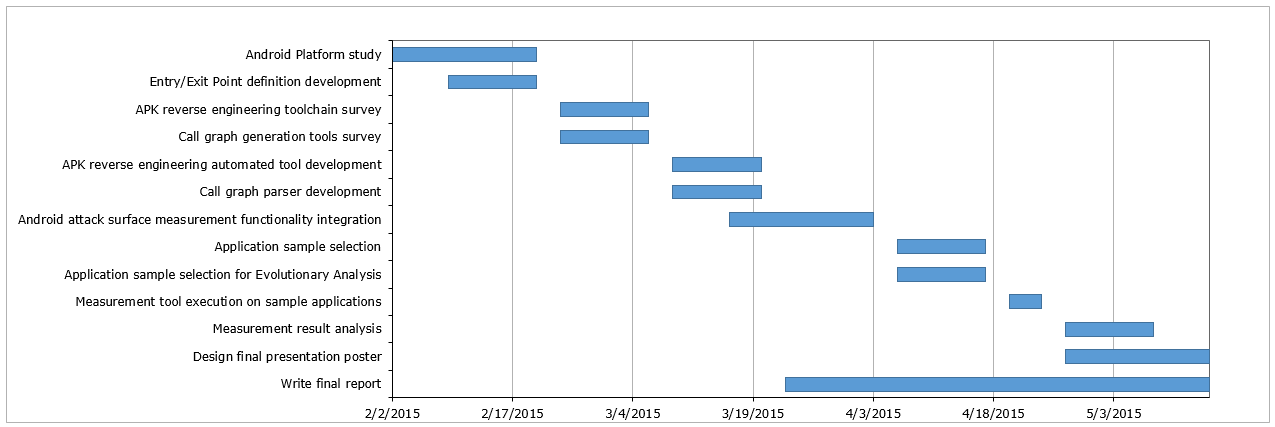
\includegraphics[scale=0.45]{figs/schedule.png}
  \caption{Project work schedule}
  \label{fig:schedule}
\end{figure*}

Figure \ref{fig:schedule} and Table \ref{tab:schedule} show the plan of work with all the project's activities with assigned beginning and finishing dates.


% An example of a floating figure using the graphicx package.
% Note that \label must occur AFTER (or within) \caption.
% For figures, \caption should occur after the \includegraphics.
% Note that IEEEtran v1.7 and later has special internal code that
% is designed to preserve the operation of \label within \caption
% even when the captionsoff option is in effect. However, because
% of issues like this, it may be the safest practice to put all your
% \label just after \caption rather than within \caption{}.
%
% Reminder: the "draftcls" or "draftclsnofoot", not "draft", class
% option should be used if it is desired that the figures are to be
% displayed while in draft mode.
%
%\begin{figure}[!t]
%\centering
%\includegraphics[width=2.5in]{myfigure}
% where an .eps filename suffix will be assumed under latex, 
% and a .pdf suffix will be assumed for pdflatex; or what has been declared
% via \DeclareGraphicsExtensions.
%\caption{Simulation Results.}
%\label{fig_sim}
%\end{figure}

% Note that IEEE typically puts floats only at the top, even when this
% results in a large percentage of a column being occupied by floats.


% An example of a double column floating figure using two subfigures.
% (The subfig.sty package must be loaded for this to work.)
% The subfigure \label commands are set within each subfloat command,
% and the \label for the overall figure must come after \caption.
% \hfil is used as a separator to get equal spacing.
% Watch out that the combined width of all the subfigures on a 
% line do not exceed the text width or a line break will occur.
%
%\begin{figure*}[!t]
%\centering
%\subfloat[Case I]{\includegraphics[width=2.5in]{box}%
%\label{fig_first_case}}
%\hfil
%\subfloat[Case II]{\includegraphics[width=2.5in]{box}%
%\label{fig_second_case}}
%\caption{Simulation results.}
%\label{fig_sim}
%\end{figure*}
%
% Note that often IEEE papers with subfigures do not employ subfigure
% captions (using the optional argument to \subfloat[]), but instead will
% reference/describe all of them (a), (b), etc., within the main caption.


% An example of a floating table. Note that, for IEEE style tables, the 
% \caption command should come BEFORE the table. Table text will default to
% \footnotesize as IEEE normally uses this smaller font for tables.
% The \label must come after \caption as always.
%
%\begin{table}[!t]
%% increase table row spacing, adjust to taste
%\renewcommand{\arraystretch}{1.3}
% if using array.sty, it might be a good idea to tweak the value of
% \extrarowheight as needed to properly center the text within the cells
%\caption{An Example of a Table}
%\label{table_example}
%\centering
%% Some packages, such as MDW tools, offer better commands for making tables
%% than the plain LaTeX2e tabular which is used here.
%\begin{tabular}{|c||c|}
%\hline
%One & Two\\
%\hline
%Three & Four\\
%\hline
%\end{tabular}
%\end{table}


% Note that IEEE does not put floats in the very first column - or typically
% anywhere on the first page for that matter. Also, in-text middle ("here")
% positioning is not used. Most IEEE journals/conferences use top floats
% exclusively. Note that, LaTeX2e, unlike IEEE journals/conferences, places
% footnotes above bottom floats. This can be corrected via the \fnbelowfloat
% command of the stfloats package.



% \section{Conclusion}
% The conclusion goes here.




% conference papers do not normally have an appendix


% use section* for acknowledgement
% \section*{Acknowledgment}


% The authors would like to thank...





% trigger a \newpage just before the given reference
% number - used to balance the columns on the last page
% adjust value as needed - may need to be readjusted if
% the document is modified later
%\IEEEtriggeratref{8}
% The "triggered" command can be changed if desired:
%\IEEEtriggercmd{\enlargethispage{-5in}}

% references section

% can use a bibliography generated by BibTeX as a .bbl file
% BibTeX documentation can be easily obtained at:
% http://www.ctan.org/tex-archive/biblio/bibtex/contrib/doc/
% The IEEEtran BibTeX style support page is at:
% http://www.michaelshell.org/tex/ieeetran/bibtex/
\bibliographystyle{IEEEtran}
\bibliography{capstone}
%
% <OR> manually copy in the resultant .bbl file
% set second argument of \begin to the number of references
% (used to reserve space for the reference number labels box)



% that's all folks
\end{document}


